Der Genetische Algorithmus(GA) wird zur Optimierung der Hyperparameter von künstlichen neuronalen Netze benutzt, da der GA in großen Suchräumen effizient arbeitet. Ein Nachteil des GA ist der hohe Rechenaufwand, weshalb im Konzept- und Implementierungsteil die Rechenzeiten beachtet werden. Um ein Konzept zu entwickeln, werden zuerst die Anforderungen an den GA definiert. Darauf aufbauend wird das Konzept des Genetischen Algorithmus erläutert. Abschließend wird auf das Konzept der Evaluierung und auf die Auswertung eingegangen.

\section{Anforderungen}
Um einen Genetischen Algorithmus umzusetzen, sind folgende Anforderungen an die Arbeit gestellt:
\begin{itemize}
\item Automatisches Trainieren eines künstlichen neuronalen Netzes
\item Automatisches Evaluieren dieser Netze
\item Automatisches Speichern der Ergebnisse
\item Automatischen Auswerten der Ergebnisse
\end{itemize}
Diese Anforderungen sind zur Umsetzung des Genetischen Algorithmus essentiell. Um den GA zu evaluieren, ist ein Algorithmus zum Vergleichen notwendig. Für diesen wurde die Zufallssuche ausgewählt, da dieser in der Literatur zur Optimierung der Hyperparameter empfohlen wird. Für beide Algorithmen gelten die gleichen, genannten Anforderungen, weshalb die spätere Implementierung möglichst modular aufgebaut wird. Somit entstehen aussagekräftige Ergebnisse, die abschließend verglichen und ausgewertet werden.  

\section{Genetischer Algorithmus} \label{ssec:GA}
Für die Anwendung der genetischen Algorithmen zur Optimierung von Hyperparametern von KNN's, wird im Folgenden ein Konzept vorgestellt. Dieses basiert auf den in Kapitel \ref{Genetische_Algorithmen} beschriebenen 5 Schritten:\\
\begin{enumerate}
  \item Initialisieren der Anfangspopulation
  \item Fitness berechnen mit Hilfe der Fitnessfunktion
  \item Selektieren der Eltern
  \item Vermehren durch Crossover und Mutation
  \item Neue Generation
\end{enumerate}
Diese Schritte sind in Abbildung \ref{fig:Ablauf_kurz} als Flussdiagramm dargestellt. Um den Genetischen Algorithmus zur Optimierung von Hyperparametern zu verwenden, werden als Gene die Hyperparameter des künstlichen neuronalen Netzes eingesetzt. Somit steht ein Individuum für ein künstliches neuronales Netz mit speziellen Hyperparametern. Dies ist in Abbildung \ref{fig:gene_hyperparameter} zu sehen. Hierdurch  werden die Gene bzw. Hyperparameter über Generationen (mehrere Iterationen) optimiert, so dass die Klassifikationsgenauigkeit steigt. Außerdem wird geprüft, inwiefern sich der Genetische Algorithmus zur Optimierung der Modell-Architektur eignet. Der Fokus der Arbeit liegt auf der Optimierung der klassischen Hyperparameter: Lernrate, Dropout, Epochen, Batchsize, Optimierer. Diese sind im Grundlagenkapitel \ref{sec:Grundlagen_Hyperparamete} definiert worden. In der Literatur wird kein Aussage zur Funktionstauglichkeit der Methoden getätigt, weswegen Experimente zu ihrer Funktionstauglichkeit durchgeführt werden. In diesen Experimenten wird der GA zur Optimierung der Hyperparameter eines künstlichen neuronalen Netzes zur Bildklassifizierung eingesetzt. Das Experiment, sowie die exakt implementierten Methoden, werden in Kapitel \ref{ssec:implementierung} detailliert beschrieben. Nachfolgend werden die Konzepte der einzelnen Schritte erläutert. Das Wissen zu den Grundlagen der Schritte und der Methoden des Genetischen Algorithmus wird für dieses Kapitel als vorausgesetzt angenommen und kann im Grundlagenkapitel \ref{Genetische_Algorithmen} nachgelesen werden.

\begin{figure}[H]
  \centering  
  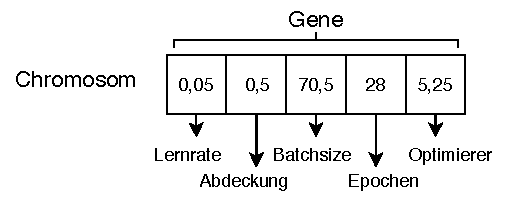
\includegraphics[scale=1.3]{img/gene_hyperparameter.pdf}
  \caption{Beispielhafte Zeichnung des Chromosoms eines Individuums, in dem die Hyperparameter als Gene realisiert wurden}
  \label{fig:gene_hyperparameter}
\end{figure}

\subsection{Initialisierung der Anfangspopulation}
Die Anfangspopulation wird zufällig innerhalb eines bestimmten Wertebereichs initialisiert. Die jeweiligen Wertebereiche sind für jeden HP individuell und müssen durch Experimente bestimmt werden. Wenn dieser Wertebereich nicht eingehalten wird, kann es dazu führen, dass die trainierten künstlichen neuronalen Netze nicht brauchbar sind. Anschließend wird die Anfangspopulation zufällig, in einem für jeden Hyperparameter speziellen Rahmen initialisiert. Diese Randbedingungen beschränken den Suchraum gezielt. Gleichzeitig müssen sie so gewählt werden, dass alle zielführenden Lösungen enthalten sind. Durch die Reduzierung des Suchraums, gestaltet sich die anschließende aufwändige Berechnung effektiver. Die exakte Größe der Population sowie die Rahmenvorgaben der Hyperparemeter wird im Implementierungsteil \ref{implementierung_init} angeführt und begründet.

\subsection{Fitnessfunktion}
Die Fitnessfunktion ermittelt die Performance der Individuen, bezogen auf ihre Aufgabe. Das Maß mit dem die Performance gemessen wird, wird als Fitnesswert bezeichnet. Bei der Optimierung von Hyperparametern ist der Fitnesswert mit der Genauigkeit der Klassifikation auf dem Testdatensatz gleichzusetzen. Es soll versucht werden, die Genauigkeit zu Maximieren, wobei das Maximum der Genauigkeit bei 1 liegt. Dementsprechend ist die Fitnessfunktion, das Trainieren eines Netzes mit den entsprechenden Hyperparametern und einem anschließendem Zurückgeben der Klassifizierungsgenauigkeit. Die exakte Fitnessfunktion wird im Implementierungskapitel \ref{implementierung_Fitnessfunktion} definiert. Darüber hinaus sollen Versuche durchgeführt werden, in denen der Fitnesswert nicht nur von der Klassifizierungsgenauigkeit abhängt, sondern aus einer Kombinationen von Interferenzgeschwindigkeit und Klassifikationsgenauigkeit. Somit könnten Modell-Architekturen für spezielle Anwendungen mit schneller Performance oder schnellem Training gefunden werden.

\subsection{Selektion der Eltern}
Zum Erstellen einer neuen Population müssen erst die Eltern ausgesucht werden. Da in der Literatur keine bestimmte Selektion der Eltern favorisiert wird. Werden im Rahmen der Arbeit für die Eltern Selektion die Fitness proportional Selektion und die Ranking Selektion verglichen. Die Methode mit den besten Ergebnissen wird anschließend zur Evaluation eingesetzt. Bei diesen Methoden handelt es sich um die State-of-the-Art Methoden, die im Grundlagen Kapitel \ref{Grundlagen_eltern_selektion} beschrieben wurden. Die verwendeten Methoden werden im Implementierungskapitel \ref{implementierung_Selektion_Eltern} beschrieben.

\subsubsection{Vermehrung}
Nachdem die Eltern Ausgewählt sind, können aus diesen die neue Generation erstellt werden, dazu kommen die zwei Methoden Crossover und Mutation zur Anwendung. Auf unterschiedlichen Umsetzungen der Methoden wird im Kapitel \ref{Grundlagen_vermehrung} eingegangen. Für die Methoden des Crossovers gibt es in der Literatur keine Aussagen über ihre Funktionstauglichkeit, weshalb für das \textbf{Crossover} die Ein-Punkt-Crossover gegenüber Zwei-Punkt-Crossover und Uniform-Crossover verglichen werden. Als \textbf{Mutation} wird eine zufällige Mutation mit einer Normalverteilung benutzt. Die verwendeten Methoden werden im Implementierungskapitel \ref{implementierung_vermehrung} beschrieben.

\subsection{Neue Generation}
Mit Hilfe der zuvor durchgeführten vier Schritten wurden die neue Individuen ausgewählt. Diese bilden die neue Generation, welche die alte Generation austauscht. Die Größe der neuen Populationen entspricht der Anfangspopulation. Um die Optimierung zu verbessern, wird geprüft, ob die Übernahme einzelner Individuen vorteilhaft ist. Die Optimierung kann nach dem Austauschen der Generationen erneut durchgeführt werden. Die 5 Schritte können für beliebig viele Generationen erfolgen oder bis zum Erreichen eines bestimmten Fintesswerts durchgeführt werden. 


\section{Evaluierungs- und Auswertungskonzept}
Für diese Arbeit ist eine ausführliche Evaluation und Auswertung essentiell. Daher ist es wichtig ein Konzept zur späteren Evaluierung und Auswertung zu entwickeln. Dieses wird speziell auf die Algorithmen der Arbeit angepasst. Nachfolgend wird auf die Konzepte der Evaluierungen der Methoden und Optimierung eingegangen.

\subsection{Evaluierung der Optimierung}
Um den Genetischen Algorithmus zur Optimierung der Hyperparameter zu evaluieren, werden die Ergebnisse des GA mit den Ergebnissen der Zufallssuche gegenübergestellt. Um eine Gegenüberstellung durchführen zu können, müssen die Laufzeiten der Algorithmen gleich gesetzt werden. Dies ist über die Trainingsvorgänge möglich, da diese 95\% der Rechenzeit beanspruchen. Die genaue Bestimmung der Iterationen wird in Kapitel \ref{sec:Evaluierung} beschrieben. Darüber hinaus wird die Optimierung an zwei verschiedenen Netzen durchgeführt, damit ein aussagekräftiges Ergebnis zustande kommt. Des Weiteren wird eine Optimierung mit kleinen Datensätzen durchgeführt. Hierbei wird geprüft, ob sich die Optimierung der Hyperparameter, mit der Optimierung von großen Datensätzen unterscheidet. 

\subsection{Auswertung}
Alle Ergebnisse werden automatisch mit den dazugehörigen Konfigurationen und Berechnungen in einer Datei abgespeichert. Aus dieser Datei wird dann automatisch eine Zusammenfassung aller Ergebnisse erstellt. Zudem sollen aus den Ergebnissen Diagramme erstellt werden, welche eine intuitive Auswertung ermöglichen.

\newpage

\section{Zusammenfassung}
In diesem Kapitel wurde das Konzept zur Optimierung der Hyperparameter von künstlichen neuronalen Netzen vorgestellt. Zuerst wurden die Anforderungen für die Arbeit bestimmt. Die Idee besteht darin die Hyperparameter als Gene des Genetischen Algorithmus umzusetzen. Somit steht jedes Individuum für ein KNN mit speziellen Hyperparametern. Diese Gene bzw. Hyperparameter werden mit Hilfe von Crossover und Mutationen über Generationen optimiert. Somit sollten bessere Ergebnisse bei der Klassifizierung von Bilddaten geliefert werden. Zudem wird die Optimierung für zwei unterschiedliche Datensätze und Netze eingesetzt, wodurch ein aussagekräftiges Ergebnis entsteht. Des Weiteren werden die Ergebnisse automatisch mit ihren dazugehörigen Konfigurationen abgespeichert und ausgewertet. 